%%%%% Définition paramètres documents

\documentclass[a4paper, 12pt]{report} % Initilisation document

% Paramètres texte

\usepackage[utf8]{inputenc} 	% Français avec caractères spéciaux
\usepackage[french]{babel}	% Français pour la biographie
\usepackage[T1]{fontenc} % Polices d'écriture

% Mise en page

\usepackage{bookmark}
\usepackage[left=2cm, right=2cm, top=2cm, bottom=2cm]{geometry} % Dimensions marges
\usepackage{indentfirst}
\usepackage{underscore}
\usepackage{nopageno} % Supprimer la pagination d'une page
\usepackage{float, caption}	% Positionnement et légende des images
\usepackage{fancyhdr}		% Marges
\usepackage{calc,ifthen,xspace}	% Redéfinition des espaces et distances

% Paramètres mathématiques

\usepackage{amsmath}
\usepackage{amssymb}
\usepackage{babel}
\usepackage{amsthm}
\usepackage{amsfonts}
\usepackage{amssymb}

% Paramètres graphiques

\usepackage{graphicx} % Inclusion images
\usepackage{epic,eepic}		% Positionnement image de garde
\usepackage{wrapfig}		% Images sur le coté dans le texte

% Autres

\usepackage{hyperref}		% Liens croisés fichier PDF
\usepackage{color}		% Couleur codes informatiques
\usepackage{lastpage}		% Références aux pages

% Identation automatique

\setlength{\parindent}{0pt} % Supression des alinéas

% Paramètres hyperliens

\hypersetup{
dvips,
backref=true,
pagebackref=true, % Bibliographies
hyperindex=true, % Index.
colorlinks=true, % Couleur hyperliens
breaklinks=true, % Retour à la ligne dans les hyperliens trop longs
urlcolor= blue, % Couleur des hyperliens
linkcolor= black, % Couleur des liens internes
bookmarks=blue, % Signets pour Acrobat
bookmarksopen=true} 

% Paramètres couleurs

\definecolor{hellgelb}{rgb}{1,1,0.8} % Codes et
\definecolor{colKeys}{rgb}{0,0,1}
\definecolor{colIdentifier}{rgb}{0,0,0}
\definecolor{colComments}{rgb}{0,0.5,0}
\definecolor{colString}{rgb}{0.62,0.12,0.94}
\definecolor{INSA_GM}{cmyk}{0.6,0,0,0} % Page de garde
\definecolor{INSA_GRIS}{cmyk}{0.7,0.6,0.5,0.3}
\definecolor{INSA_BLEU}{cmyk}{1,0.9,0.1,0}

% 

\newcommand{\insertrefproj}[1]{}
\newcommand{\refproj}[1]{\renewcommand{\insertrefproj}{\textbf{\color{INSA_GRIS}#1}}}

% Style de page

\pagestyle{fancy}

\fancypagestyle{courant}{
	\fancyhf{}
    \setlength{\headheight}{27pt}
    \fancyhead[L]{\raisebox{-2mm}{
\includegraphics[width=30mm]{Images/Logo INSA.png}}}
\fancyhead[C]{}
\fancyhead[R]{\color{INSA_GRIS}\thepage}%\scshape\leftmark}
\fancyfoot[L]{\insertrefproj}
\fancyfoot[R]{}
%\fancyfoot[CE,CO]{\color{INSA_GRIS}\thepage}
\renewcommand{\headrulewidth}{0pt}
\renewcommand{\footrulewidth}{0.2pt}
}

\fancypagestyle{special}{%
  \pagestyle{courant}
  \fancyfoot{}
  %\addtolength{\footskip}{-20pt}
%  \setlength{\footskip}{0pt}
%  \fancyfoot[C]{}
\renewcommand{\footrulewidth}{0pt}
}

\fancypagestyle{plain}{%
  \fancyhf{}%
  \pagestyle{courant}
}

% 

\newcommand{\Scilab}{
	\lstset{
	language=Scilab,
	float=hbp,
	basicstyle=\ttfamily\small,
	identifierstyle=\color{colIdentifier},
	keywordstyle=\bf \color{colKeys},
	stringstyle=\color{colString},
	commentstyle=\color{colComments},
	columns=flexible,
	tabsize=5,
	frame=single,
	%frame=shadowbox,
	rulesepcolor=\color[gray]{0.5},
	extendedchars=true,
	showspaces=false,
	showstringspaces=false,
	numbers=left,
	stepnumber=5,
	firstnumber=1,
	numberstyle=\tiny,
	breaklines=true,
	%backgroundcolor=\color{hellgelb},
	captionpos=b,
	}
}

% Paramètres projet

\title{Projet de P6}
\refproj{STPI/P6/2024 - 39}
\author{}
\date{}

%%%%% Début d'édition du document

\begin{document}

%%% Page de présentation

\pagenumbering{Alph} % Numérotation
\thispagestyle{empty} % Type page

\vspace{4cm}

\begin{picture}(0,0) % Hauteur , Largeur
	
\put(80,-465){\includegraphics[scale=1]{images/Image Garde.png}} % Image de garde centrée horizontalement
\put(0,-20){
\includegraphics[width=0.4\textwidth]{images/Logo INSA.png}} % Logo INSA haut-gauche
\put(240,0){{\begin{minipage}{12cm}\centering \Large % Caractéristiques projet haut droit
	\textbf{Projet de Physique P6} \\ 
	\textbf{STPI/P6/2024 - 39}\end{minipage}}}
\put(-20,-150){{\begin{minipage}{\textwidth}\centering \Huge % Titre princpal rapport
	\textbf{Modélisation de l'impact des gaz à effet de serre}\end{minipage}}}
% Quelques changements pour illustrer
\newsavebox{\noms}
\savebox{\noms}(300, 300)[tl]{
\put(0,98){\color{INSA_GRIS}{\begin{minipage}{6cm} 
	\textbf{Étudiants :} \end{minipage}}} % Étudiants par ordre alphabétique de prénom
\put(0,60){\color{INSA_GRIS}{\begin{minipage}{6cm}
	Romane LANÈRES \\ Anouk PETITGAS \\ Arthur SARRAU \end{minipage}}}
\put(185,60){\color{INSA_GRIS}{\begin{minipage}{6cm}
	Clara MÉLINE \\ Tom PHILIPPE \\ Nina ZEDDOUN \end{minipage}}}

\put(0,){\color{INSA_GRIS}\begin{minipage}{9cm}   
	\textbf{Enseignant-responsable du projet :} \\ Samuel PAILLAT \end{minipage}}}

\put(100,-850){\usebox{\noms}}

\end{picture}

%%% Page complètement vierge

\newpage
\pagenumbering{arabic}
\setcounter{page}{1}
\thispagestyle{empty}
\null

%%% Page descriptions cractéristiques principales projet

\newpage
\pagestyle{special}

\textbf{Date de remise du rapport :} 13/06/2024 \\

\textbf{Référence du projet:} STPI/P6/2024 – 39 \\

\textbf{Intitulé du projet :} Modélisation de l'impact des gaz à effet de serre \\

\textbf{Type de projet :} Modélisation numérique \\

\textbf{Objectifs du projet :} \\ 

Ce projet a pour vocation de développer un modèle numérique 
décrivant les mécanismes de régulation thermique de 
l'atmosphère terrestre. Premièrement, nous allons réaliser
une étude à travers quelques calculs en ordre de grandeurs afin
d'identifier les différents paramètres d'influence de notre modèle.
L'objectif est de mettre au point un modèle qui soit modulable
en termes de paramètres et de complexité. Cette dernière est 
ajustée par le traitement de différents gaz à effet de serre 
et de divers modèles de température et de pression. 
L'ensemble des modélisations numériques aspire à proposer 
une version améliorée du travail réalisé par le 
vulgarisateur scientifique David Louapre. À travers ce projet, 
nous cherchons à reproduire au mieux le 
phénomène d'équilibre thermique de la Terre en considérant 
les flux principaux et en quantifiant précisément l'impact
des gaz à effet de serre dans le système atmosphérique. \\

\textbf{Mots-clefs du projet :} Transfert thermique, Corps noir, Effet de serre, Bilan radiatif \\ 

\vfill

% Coordonnées INSA Rouen par défaut

\begin{center}
	\scshape Institut National des Sciences Appliquées de Rouen \\
	Département Sciences et Techniques Pour l'Ingénieur \\
	685 Avenue de l'Université BP 08- 76801 Saint-Etienne-du-Rouvray \\ Tél : 33 2 32 95 66 21 - Fax : 33 2 32 95 66 31
\end{center}

%%% Remerciements

\newpage
\chapter*{Remerciements} % Garde la même mise en page qu'un chapitre mais ne le numérote pas
\addcontentsline{toc}{chapter}{Remerciements} % Ajout dans le sommaire, possiblement renommé comme souhaité

\setlength{\parindent}{30pt}
Nous souhaiterions avant tout remercier Samuel PAILLAT, notre
coordinateur et enseignant encadrant, qui a su nous aiguiller
et nous apporter son aide et ses connaissances tout au longs
de ce projet. \\

\indent Aussi nous aimerions nous porter reconnaissants 
envers le physicien médaillé de la médiation scinetifique
du CNRS: David Louapre. Ces travaux sur l'effet de serre 
ont été une grande source d'inspiration en tant que point 
de départ pour notre recherche. \\

\indent Nous saluons également les divers organismes ayant 
mis à disposition des bases de données en open source. Nous
en avons extrait des paramètres physiques sans lesqueles 
nos modèles auraient manqué de fiabilité. \\

\indent Enfin, nous aimerions remercier l'organisation de 
l'INSA plus généralement pour nous avoir implémenté l'EC de P6
qui nous a permis de réaliser notre premier projet
scientifique appliqué dans des conditions de collaboration
collective proches de celle milieu de l'ingénierie. 
\vfill


%%% Table des matières 

\newpage
\pagestyle{courant} 
	\setcounter{tocdepth}{2} % Règle la profondeur maximale de la table des matières
	\tableofcontents % Affichage table des matières

%%% Notations et Acronymes

\newpage
\chapter*{Notations et Acronymes} 
\addcontentsline{toc}{chapter}{Notations et Acronymes}

\begin{description}
	\item[GES:] Gaz à Effet de Serre
    \item[CN:] Corps noir
    \item[\Phi:] FLux 
\end{description}

%%% Introduction

\newpage
\chapter*{Introduction}				
\addcontentsline{toc}{chapter}{Introduction}

Ce dernier se base principalement 
sur la physique des transferts thermiques, mais fait également
appel à des compétences en informatique et mathématiques. 
\begin{itemize}
\item Contexte du travail
	  
\item Objectifs à atteindre pour le projet
\end{itemize}

%%% Méthodologie, organisation du travail

\chapter{Méthodologie, organisation du travail}

\begin{itemize}
\item Description de l’organisation adoptée pour le déroulement du travail
\item Organigramme des tâches réalisées et des étudiants concernés
\end{itemize}

%%% Travail réalisé et résultats

\chapter{Travail réalisé et résultats}

	\section{L'effet de serre}

		\subsection{Explication du phénomène de l'effet de serre}


L’effet de serre est un processus naturel qui se produit avec le rayonnement entre la Terre et le Soleil. Tout d'abord, le soleil émet un rayonnement vers la Terre, l'atmosphère laisse passer une partie de ce rayonnement solaire. Réchauffé, le corps terrestre, étant un corps noir, émet un flux rayonné identique à celui reçu par soleil. Ce flux est alors renvoyé vers l'atmosphère et une partie est absorbée par les gaz présents , appelés gaz à effet de serre . Le reste du flux est soit envoyé dans l'espace, soit renvoyé vers la Terre. 
De plus, nous avons pu constater que ce phénomène n'existe que lorsque que la température varie dans l'atmosphère en fonction de l'altitude. Ainsi si la température était uniforme dans l'atmosphère ce phénomène n'existerait pas. 
\begin{figure}[!ht]
\centering
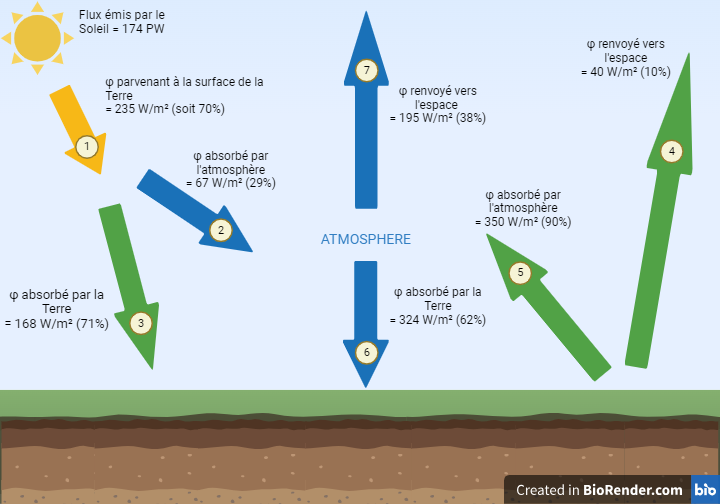
\includegraphics[width=15cm]{schemaflux.png}
      \caption{Schéma du phénomène de l'effet de serre}   
%\vspace{-2.cm} 
\end{figure}

C'est l'absorbtion du rayonnement par les GES qui va provoqué un rechauffement terrestre. Ainsi, ce phénomène créé un réchauffement global de la Terre permettant à la température moyenne de s'éléver à 15°C au lieu de -18°C (sans GES).    

        \subsection{Définition des GES}
gaz à effet de serre (source gouvernement) : gaz présent dans l’atmosphère qui retient une partie de la chaleur reçue par le solaire dans l’atmosphère. Certains gaz sont d’origine naturelle (vapeur d’eau, par exemple) et/ou issues des activités humaines, en particulier les gaz fluorés.
présents naturellement dans l’atmosphère (vapeur d’eau, dioxyde de carbone,...), la Terre absorbe une partie de l’énergie qu’elle reçoit du soleil, le reste étant renvoyé vers l’espace. \\

\begin{figure}[h]
\centering
\vspace{-0.6cm} 
%\includegraphics[width=0.62\linewidth]{PistonHeatReservoir.pdf}

\includegraphics[width=43mm]{Images/Logo INSA.png}\captionof{figure}[LogoINSA]{Super Logo}
%\vspace{-2.cm} 
\end{figure}



	Lorem ipsum dolor sit amet, consectetuer adipiscing elit. Sed non risus. Suspendisse lectus tortor, dignissim sit amet, adipiscing nec, ultricies sed, dolor. Cras elementum ultrices diam. Maecenas ligula massa, varius a, semper congue, euismod non, mi. Proin porttitor, orci nec nonummy molestie, enim est eleifend mi, non fermentum diam nisl sit amet erat. Duis semper. Duis arcu massa, scelerisque vitae, consequat in, pretium a, enim. Pellentesque congue. Ut in risus volutpat libero pharetra tempor. Cras vestibulum bibendum augue. Praesent egestas leo in pede. Praesent blandit odio eu enim. Pellentesque sed dui ut augue blandit sodales. Vestibulum ante ipsum primis in faucibus orci luctus et ultrices posuere cubilia Curae; Aliquam nibh. Mauris ac mauris sed pede pellentesque fermentum. Maecenas adipiscing ante non diam sodales hendrerit.\\

%Si vous voulez numéroter les équations faîtes ceci : 
\begin{equation}
	y = a x + b
\end{equation}
%Sinon mettez juste $$ y = ax + b $$

				\subsubsection{Conseils de rédaction}

	Le rapport ne devra pas dépasser un nombre maximum de \textbf{20 pages} (hors annexes). Les informations attendues dans ce rapport sont données ci-dessous. Toutefois, l’organisation et les intitulés des chapitres sont laissés au libre choix des étudiants. La mise en page de ce document est à respecter. 

	\chapter*{Conclusion et perspectives}		% garde la même mise en page qu'un chapitre mais ne le numérote pas
	\addcontentsline{toc}{chapter}{Conclusion et perspectives}% permet de l'avoir dans le sommaire
\begin{itemize}
\item Conclusions sur le travail réalisé
\item Conclusions sur l'apport personnel de cte E.C. projet
\item Perspectives pour la poursuite de ce projet
\end{itemize}

\begin{thebibliography}{9}
	\addcontentsline{toc}{chapter}{Bibliographie}	% permet de l'avoir dans le sommaire

	\bibitem{Livre 01}
		\textsc{Nom}, Prénom
		\textit{Titredu livre },
		Editeur, Année.

	\bibitem{Article 01}
		\textsc{Nom des Auteurs},
		"\textit{Titre de l'article}",
		Titre du journal,
		Volume, pages, année.

	\bibitem{Lien Internet 01}
\textsc{lien Internet},
		\url{http://www.\#\#\#\#}
		(Valide à la date du \#\#/\#\#/201\#)

\end{thebibliography}

\appendix

	\chapter{Documentation technique}

Les annexes ne sont pas obligatoire, les annexes présentées ici le sont à titre indicatif.
	\chapter{Listings des programmes réalisés}
	\chapter{Schémas de montages, \\plans de conception...}
	\chapter{Propositions de sujets de projets \\ (en lien ou pas avec le projet réalisé)}
	\chapter{Mettre du code en annexe}

	Voici comment mettre du code source en annexe. Attention ! Les accents et caractères spéciaux ne sont pas pris en compte pour l'insertion de code.

\end{document}
